\documentclass[10pt]{beamer}

\usetheme[progressbar=frametitle, block=fill]{metropolis}
\usepackage{xcolor}
\usepackage{multirow}
\usepackage{pgfpages}
\usepackage{pifont}
\usepackage[utf8]{inputenc}
\usepackage[T1]{fontenc}
\usepackage[english]{babel}
\newcommand{\cmark}{\ding{51}}
\newcommand{\xmark}{\ding{55}}
\setbeamertemplate{note page}{\insertnote}
%\setbeameroption{show notes on second screen=left}
\setbeameroption{hide notes}
\definecolor{amethyst}{rgb}{0.5, 0.4, 1.0}
\definecolor{amethystgrey}{rgb}{0.85, 0.85, 1.0}
\definecolor{amethystdark}{rgb}{0.4, 0.3, 0.9}
\definecolor{orangedark}{rgb}{0.0, 0.9, 0}
%\definecolor{titlebg}{HTML}{4e8074}
%\definecolor{titlebg}{HTML}{3e7985}
\definecolor{titlebg}{HTML}{fbf8ff}
\definecolor{font}{HTML}{23373b}
%\setbeamercolor{title}{fg=amethyst, bg=amethyst}
\setbeamercolor{frametitle}{fg= font, bg=titlebg}
%\setbeamercolor{section title}{black}
%\setbeamercolor{structure}{fg=amethyst, bg=amethyst}
\setbeamercolor{progress bar}{ fg = amethyst, bg= amethystgrey }
%\setbeamercolor{itemize item}{fg=amethyst,bg=white}
\setbeamercolor{alerted text}{fg=amethystdark}
%\setbeamercolor{title separator}{ ... }
%\setbeamercolor{progress bar in head/foot}{ ... }
%\setbeamercolor{progress bar in section page}{ ... }

\usepackage{booktabs}
\usepackage[scale=2]{ccicons}

\usepackage{minted}

\usepackage{pgfplots}

\usepackage{xspace}

\title{[l, gl, x, r, pr]values}
\subtitle{Value categories}
\date{}
\author{Dawid Pilarski}
\institute{dawid.pilarski@tomtom.com}

\begin{document}

\maketitle

\section{Introduction}

\begin{frame}{How are expressions categorized?}
\centering
	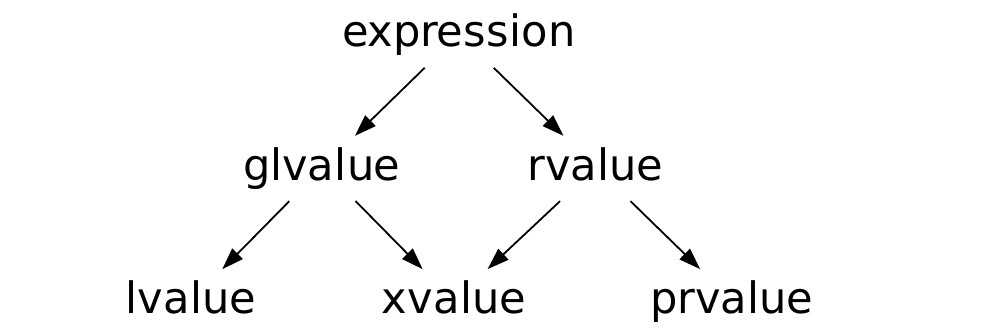
\includegraphics[width=\linewidth]{value_categories-1.jpg}
\end{frame}

\begin{frame}{How to understand fundamental classifications?}
	\begin{itemize}
		\item lvalue - T\& \pause
		\item xvalue - T\&\& \pause
		\item prvalue - T
	\end{itemize}
\end{frame}

\begin{frame}{The common mistake}
	\centering
	Usually people think about expression categories: \\ 
	\vskip 3em
	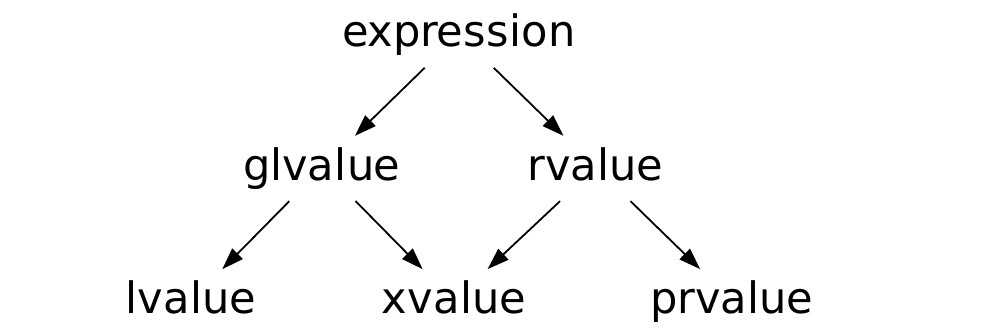
\includegraphics[width=0.5\linewidth]{value_categories-1.jpg} \\
		\vskip 3em As categories of references, which is \alert{\color{red}wrong}
\end{frame}

\begin{frame}{Getting it right}
	\centering
	expression \alert{belongs to} category \\
	reference \alert{determines} category \\
	category \alert{does not determine} reference\\
	
	\vfill
	
	\footnotesize
	[Note: there is no reference of type prvalue]
\end{frame}

\begin{frame}{Why categorization?}
Different value categories:
\begin{itemize}
	\item Different \alert{conversion rules}
	\item Different \alert{requirements on types}
	\item Different \alert{behavior}
\end{itemize}
\end{frame}


\begin{frame}{prvalue vs glvalues}
	\begin{description}
		\item[glvalues] \hfill \\ 
			Generalized lvalues. It's everything that \alert{references the \emph{object}}
		\item[prvalues] \hfill \\
			Pure rvalues. It's a \alert{value}.
	\end{description}
\end{frame}

\section{Into the details - glvalues}

\begin{frame}{Xvalues}
	\begin{description}
		\item[xvalues] - eXpiring values
	\end{description}

	\vskip3em

	Xvalues are such kind of expressions, that its' results point to the object,
	which will soon \alert{expire}.

\end{frame}

\begin{frame}{Xvalues examples}
	There are fixed number of ways we can get xvalues:
	\begin{itemize}
		\item function call which result type is rvalue reference (T\&\&).
		\item explicit cast to rvalue reference.
		\item subscript operator call on the xvalue arrays.
		\item non reference member access to the xvalue objects (also through pointer to member).
		\item temporary materialization conversion.
	\end{itemize}
\end{frame}

\begin{frame}[fragile]{function call which result type is rvalue reference}
	\begin{minted}{c++}
struct Foo{};
Foo&& bar(); 

int main(){
  bar(); // "bar()" is the xvalue expression 
}
	\end{minted}
\end{frame}

\begin{frame}[fragile]{explicit cast to rvalue reference}

\begin{minted}{c++}
struct Foo{/* definition */};

int main() {
  Foo a;
  std::move(a); // "std::move(a)" casts a to Foo&&
  static_cast<Foo&&>(a); // does same thing as std::move
}
\end{minted}

\end{frame}

\begin{frame}[fragile]{subscript operator call on the xvalue arrays}
	\begin{minted}{c++}
int main(){
  Foo arr[10] = {};
  std::move(arr)[0]; // xvalue ref to the first arr element
}
	\end{minted}
\end{frame}

\begin{frame}[fragile]{non reference member access  to the xvalue objects}
	\begin{minted}{c++}
template <typename T>
struct Foo{
  T member;
};

int main(){
  Foo<int> a{};
  std::move(a).member; //xvalue 
  
  Foo<int&> b{.member = a.member};
  std::move(b).member; // lvalue 
                       // (reference collapsing)
}
	\end{minted}
\end{frame}

\begin{frame}[fragile]{non reference member access  to the xvalue objects II}
	\begin{minted}{c++}
int main(){
  int Foo<int>::* pointer = &Foo<int>::member;
  Foo<int> foo{};
  std::move(foo).*pointer; //xvalue expression
  return 0;
}
	\end{minted}
\end{frame}

\begin{frame}[fragile]{temporary materialization conversion}
	\begin{minted}{c++}
struct Foo{int member;};
Foo().member; // member access requires glvalue
              // tmc converts the prvalue to xvalue
	\end{minted}
\end{frame}


\begin{frame}[fragile]{Complete type requirements}
	\centering
	glvalue expressions can operate on non-complete type
	\vskip 0.5em
	\hrule
	
	\begin{minted}{c++}
struct Foo;

Foo& first_foo();
Foo& second_foo();

Foo& first_of_two(Foo& first, Foo& second){return first;}

int main(){
  auto& result = first_of_two(second_foo(), first_foo());
  if(&result == &second_foo())
    std::cout << "result is second" << std::endl; 
}
		
	\end{minted}
\end{frame}

\begin{frame}{glvalue and void}
	expression, which result is of type void cannot be glvalue expression.
	\vskip 2em
	
	\begin{itemize}
		\item It's impossible to create object of type void
		\item It's impossible to have a reference to void
	\end{itemize}
\end{frame}

\section{into the details - prvalues}

\begin{frame}{What are prvalues expressions}
	Those are expression which results are the \alert{values}.
\end{frame}

\begin{frame}[fragile]{prvalues examples}
	\begin{minted}{c++}
	struct Foo{};
	Foo(); // returns value of type Foo.
	
	Foo bar();
	bar(); // prvalue returns type Foo
	\end{minted}
	
\end{frame}

\begin{frame}{prvalues and void}
\centering
	Prvalues expressions can return void type.
\end{frame}

\begin{frame}[fragile]{Type completeness requirements}
	\centering
	Prvalues expressions that yield type T needs this type to be complete.
	\vskip 0.5em
	\hrule
	\vfill
	
	\begin{minted}{c++}
Foo first_copy_of_two(Foo& first, Foo& second){return first;}
		
int main(){
  // call to first_of_two is now prvalue expression
  // the program will not compile
  const auto& result = first_of_two(second_foo(),
                                    first_foo());
  if(&result == &second_foo())
    std::cout << "result is second" << std::endl; 
}
	\end{minted}
\end{frame}

\section{Expression categories conversion}

\begin{frame}{Types of categories conversions}
	\begin{columns}
		\begin{column}[t]{0.45\linewidth}
			\centering
			glvalue to prvalue
			\vskip 0.5em
			\hrule
			
			\begin{itemize}
				\item array to pointer conversion
				\item function to pointer conversion
				\item lvalue to rvalue
			\end{itemize}
			
		\end{column}
		\begin{column}[t]{0.45\linewidth}
			\centering
			prvalue to glvalue
			\vskip 0.5em
			\hrule
			
			\begin{itemize}
				\item temporary materialization conversion
			\end{itemize}
		\end{column}
	\end{columns}
\end{frame}

\begin{frame}[fragile]{array to pointer conversion}
	\begin{minted}{c++}
void printme(const char* str);
int main(){
  char str[] = {'a', 'b', 'c', 'd', '\0'};
  printme(str); 
}
	\end{minted}
\end{frame}

\begin{frame}[fragile]{function to pointer}
	\begin{minted}{c++}
void foo(){} 
void foo2(void(*)()); 
void foo3(void(*)()&);

void main(){
  foo; // type void(&)() lvalue
  foo2(foo); // void(&)() -> void(*)()
  foo3(foo); // also fine
};
	\end{minted}
\end{frame}

\begin{frame}{lvalue to rvalue conversion}
	\centering
	Does not take place for:
	\begin{itemize}
		\item arrays
		\item functions
	\end{itemize}
	\vskip 3em
	For not-complete type conversion is ill-formed.
\end{frame}

\begin{frame}{lvalue to rvalue}
	\begin{itemize}
		\item for non class types the cv qualifiers are discarded
		\item for class types the cv qualifiers are preserved
	\end{itemize}
\end{frame}

\begin{frame}[fragile]{lvalue to rvalue semantics}
	\centering 
	Lvalue to rvalue conversion means \alert{reading object's value} \\
	T\& $\rightarrow$ T
	
	\vskip 0.5em
	\hrule
	\vfill
	
	\alert{\S 7.2.3.2 Expression context dependence }
	\vskip 0.75em
	
	\begin{quote}
		In some contexts, an expression only appears for its side effects.
		Such an expression is called a discarded-value expression.
		\dots \vskip 1em
		The lvalue-to-rvalue conversion is applied if and only if the expression is a glvalue of volatile-qualified type and it is one of the following:
	\end{quote}
\end{frame}


\begin{frame}[fragile]{lvalue to rvalue semantics}
	\centering 
	Lvalue to rvalue conversion means \alert{reading object's value} \\
	T\& $\rightarrow$ T

	\vskip 0.5em
	\hrule

	\begin{minted}{c++}
extern volatile int GPIO_Port;	
volatile int& foo(){ return GPIO_Port; }

int main(){
  foo();
}
	\end{minted}
\end{frame}

\begin{frame}[fragile]{lvalue to rvalue conversion}
	\begin{minted}{c++}
void foo(Bar value);
Bar bar;
foo(bar);
	\end{minted}
\end{frame}

\begin{frame}{temporary materialization conversion}
	\centering
	\begin{itemize}
		\item If glvalue expression is expected and prvalue is present.
		\item Temporary variable is created
		\item Conversion to the xvalue is applied.
	\end{itemize}
\end{frame}

\begin{frame}[fragile]{temporary materialization conversion}
	\begin{minted}{c++}
struct Foo{};	
	
void foo(Foo&& test){
  std::cout << "ptr to test: " << &test << std::endl;
}

int main()
{
  Foo* ptr = &Foo(); // ill-formed lvalue is required
  foo(Foo());
}
	\end{minted}
\end{frame}

\section{Bitfields}

\begin{frame}[fragile]{Bitfields and glvalues}
	\begin{minted}{c++}
struct Foo{
  char a:3;
};

Foo().a; // glvalue 
Foo foo;
foo.a // lvalue
auto i = foo.a; // automatic conversion to bitfield type
auto& j = foo.a; // ill formed
const auto& k = foo.a; // valid statement

	\end{minted}
\end{frame}

\begin{frame}{Thanks}
	\centering
	Thank you for attention!
	
	\vskip0.5em
	
	Questions?
	
	\vfill

\hrule
\vskip0.5em
\footnotesize
	
	\centering Bibliography
	\begin{itemize}
		\item \alert{\href{blog.panicsoftware.com}{My blog}}
		\item \alert{\href{eel.is/c++draft/}{IS draft}}
	\end{itemize}
\end{frame}

\end{document}